%%
%% Gutenberg IR Search Engine -- ACM sigconf Report
%% Author: Arun Narayanan, Dublin City University
%%
\documentclass[sigconf,nonacm]{acmart}

\usepackage{booktabs}
\usepackage{tikz}
\usetikzlibrary{positioning, shapes.geometric, arrows.meta}
\usepackage{amsmath}
\usepackage{listings}
\usepackage{xcolor}
\usepackage{hyperref}
\usepackage{enumitem}

% Allow LaTeX extra stretch to prevent monospace tokens from overflowing margins
\emergencystretch=2em
\hfuzz=5pt  % suppress overfull warnings under 5pt (sub-millimetre)

\lstset{
  basicstyle=\ttfamily\footnotesize,
  breaklines=true,
  frame=single,
  language=Python,
  keywordstyle=\color{blue},
  commentstyle=\color{gray},
}

% Remove ACM copyright block for coursework
\setcopyright{none}
\settopmatter{printacmref=false}
\renewcommand\footnotetextcopyrightpermission[1]{}
\pagestyle{plain}

\begin{document}

\title{Full-Text Search Engine for Project Gutenberg}

\author{Arun Narayanan}
\affiliation{%
  \institution{Dublin City University}
  \city{Dublin}
  \country{Ireland}
}
\email{arun.narayanan2@mail.dcu.ie}

% ============================================================
\begin{abstract}
This report presents the design, implementation, and evaluation of a full-text
search engine built entirely from scratch for the Project Gutenberg digital
library.  The system indexes 70{,}772 documents (27.8\,GB of raw text) using a
Single-Pass In-Memory Indexing (SPIMI) strategy with varint-encoded postings
stored in a dual-file architecture (SQLite metadata plus a flat binary postings
file).  Three retrieval models are supported: \emph{structured metadata search},
\emph{TF-IDF Vector Space Model (VSM)}, and \emph{Okapi BM25}, along with a
phrase-fallback mechanism that handles stopword-heavy queries where standard
bag-of-words models fail.  I evaluate the system on six benchmark queries using
manual relevance judgments and report Precision@10, Average Precision@10, and
NDCG@10 across all query-model combinations.  The results reveal that no single
model dominates all query types: structured search achieves perfect precision
for metadata-matching queries (P@10$=$1.0), while BM25 outperforms VSM on
content-oriented queries thanks to document-length normalization.  The entire
index builds in approximately 10.5 hours on a single consumer laptop (Intel
Core i7-14650HX, 16\,GB RAM) with a peak traced memory footprint of approximately 1\,GB.
\end{abstract}

\keywords{Information retrieval, inverted index, BM25, TF-IDF, SPIMI,
Project Gutenberg}

\maketitle

% ============================================================
\section{Introduction}

Information Retrieval (IR) is the task of finding relevant documents from a
large collection in response to a user's information
need~\cite{manning2008introduction}.  This project implements a search engine
over the Project Gutenberg corpus~\cite{gutenberg2024}, one of the oldest and
largest collections of public-domain e-books, containing over 70{,}000 full-text
documents in multiple languages.  The corpus snapshot used in this work was
obtained in February 2025 from the official Gutenberg mirror.

In accordance with the assignment policy, I used only Python's standard
library plus NumPy and Pandas for data handling; no external IR
frameworks (Lucene, Elasticsearch, Terrier, Solr, etc.) were used.
The project was developed under the following constraints:
\begin{enumerate}[nosep]
  \item No external IR frameworks or search libraries.
  \item Only the Python standard library plus NumPy and Pandas.
  \item Deterministic, reproducible results.
\end{enumerate}
These constraints ensure that every component of the system is implemented and
understood from first principles.\footnote{Source code and outputs:
\url{https://github.com/ArunGMR0411/gutenberg-search-engine}}

\subsection{Contributions}
The main contributions of this work are:
\begin{enumerate}[nosep]
  \item A scalable SPIMI-based inverted index with varint-encoded postings,
        supporting 22.5 million unique terms across a 27.8\,GB corpus.
  \item Three retrieval models (structured, VSM, BM25) with a phrase-fallback
        mechanism for stopword-heavy queries.
  \item A systematic comparative evaluation on six deliberately diverse queries
        with manual relevance judgments and standard IR metrics.
\end{enumerate}

\subsection{Corpus Challenges}
Several characteristics of the Gutenberg corpus make retrieval harder than
typical web or newswire collections:
\begin{itemize}[nosep]
  \item \textbf{Extreme document-length variance.}  Lengths range from a
        single sonnet ($\sim$300 tokens) to compilations like the Complete
        Works of Shakespeare ($>$900{,}000 tokens).  Bag-of-words models
        exhibit short-document bias unless lengths are properly normalized.
  \item \textbf{Boilerplate contamination.}  Every file contains a Project
        Gutenberg header and footer with licensing text.  I strip this
        boilerplate using \texttt{*** START OF} / \texttt{*** END OF}
        markers (99.96\% of files have both, measured during indexing),
        but roughly one-third of stripped files still mention ``Gutenberg''
        inside the content zone (via book titles referencing the project,
        credit lines, and self-referential URLs), which confounds Q5 retrieval.
  \item \textbf{Multilingual content.}  The corpus includes texts in English,
        German, French, Spanish, and other languages.  Query~6
        (``Dornr\"oschen'') specifically tests Unicode handling and
        accent-fold matching across scripts.
  \item \textbf{Stopword-dominated queries.}  Query~1 (``to be, or not to
        be'') consists entirely of common English words; TF-IDF models
        assign near-identical, non-discriminative weight to each token,
        producing near-tied scores and semantically meaningless rankings.
\end{itemize}

% ============================================================
\section{Related Work}

The Vector Space Model was introduced by Salton et~al.~\cite{salton1975vsm},
representing documents and queries as vectors in a high-dimensional term space
and ranking by cosine similarity.  Okapi BM25, developed by Robertson and
Walker~\cite{robertson1994okapi} and later refined into a formal probabilistic
framework~\cite{robertson2009bm25}, extended this with saturation-based term
frequency weighting and explicit document-length normalization, consistently
outperforming pure TF-IDF models in TREC
evaluations~\cite{robertson1995trec3}.

For large-scale indexing, Heinz and Zobel~\cite{heinz2003spimi} proposed
Single-Pass In-Memory Indexing (SPIMI), which processes documents sequentially
into memory-bounded blocks and merges them in a single pass.  SPIMI avoids the
term-at-a-time overhead of the traditional BSBI approach and is particularly
well-suited for corpora that exceed available RAM.

My implementation builds on these foundations: SPIMI for disk-bounded indexing,
TF-IDF cosine similarity for the VSM model, and BM25 with $k_1 = 1.2$,
$b = 0.75$.  Where my system differs is in the addition of a metadata-only
structured model and a phrase-fallback mechanism for the Gutenberg corpus.

% ============================================================
\section{System Architecture}

% System Architecture Diagram (TikZ)
% Include with: % System Architecture Diagram (TikZ)
% Include with: % System Architecture Diagram (TikZ)
% Include with: \input{figures/architecture.tex}
\begin{figure*}[t]
\centering
\resizebox{\textwidth}{!}{%
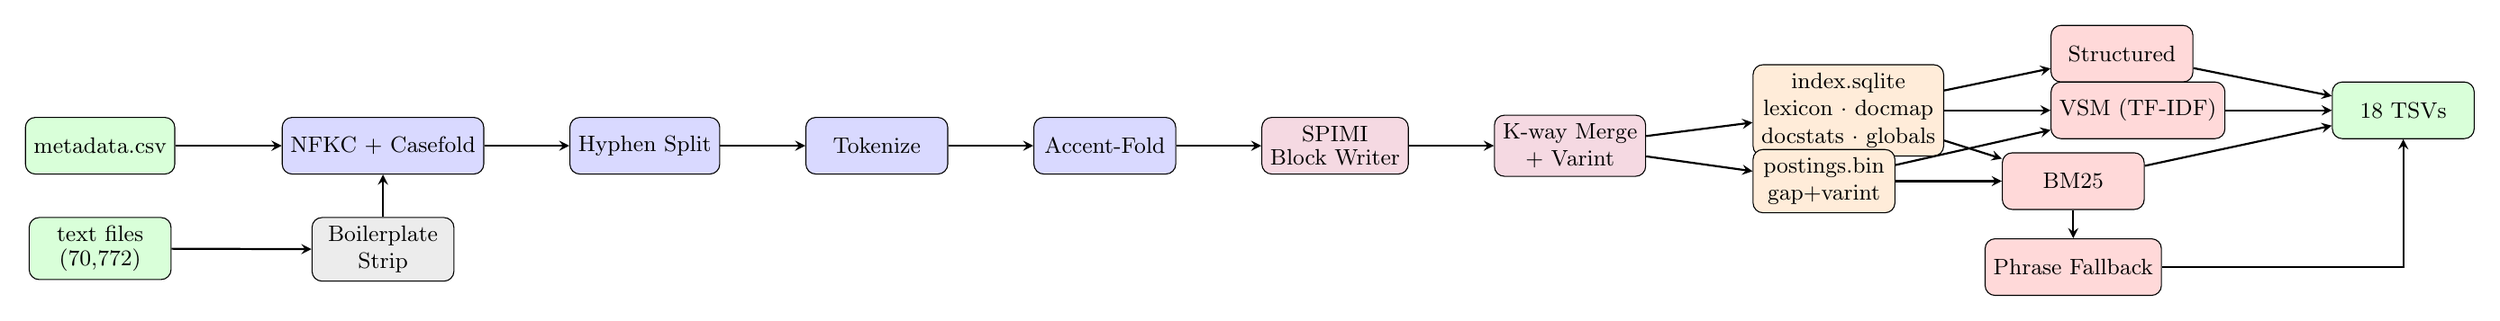
\begin{tikzpicture}[
    node distance=1.2cm and 1.5cm,
    box/.style={draw, rounded corners, minimum width=2cm, minimum height=0.8cm,
                fill=#1!15, font=\small},
    box/.default=blue,
    storage/.style={draw, minimum width=1.8cm, minimum height=0.8cm,
                    fill=orange!15, font=\small},
    arrow/.style={->, >=stealth, thick},
    label/.style={font=\footnotesize\itshape, text=gray}
]

% Input
\node[box=green] (csv) {metadata.csv};
\node[box=green, below=0.6cm of csv] (txt) {\shortstack{text files\\(70{,}772)}};

% Preprocessing
\node[box, right=1.5cm of csv] (nfkc) {NFKC + Casefold};
\node[box, right=1.2cm of nfkc] (hyph) {Hyphen Split};
\node[box, right=1.2cm of hyph] (tok) {Tokenize};
\node[box, right=1.2cm of tok] (alias) {Accent-Fold};
\node[box=gray, below=0.6cm of nfkc] (strip) {\shortstack{Boilerplate\\Strip}};

% Indexing
\node[box=purple, right=1.2cm of alias] (spimi) {\shortstack{SPIMI\\Block Writer}};
\node[box=purple, right=1.2cm of spimi] (merge) {\shortstack{K-way Merge\\+ Varint}};

% Storage
\node[box=orange, right=1.5cm of merge, yshift=0.5cm] (sqlite)
    {\shortstack{index.sqlite\\lexicon $\cdot$ docmap\\docstats $\cdot$ globals}};
\node[box=orange, right=1.5cm of merge, yshift=-0.5cm] (bin)
    {\shortstack{postings.bin\\gap+varint}};

% Retrieval
\node[box=red, right=1.5cm of sqlite, yshift=0.8cm] (struct) {Structured};
\node[box=red, right=1.5cm of sqlite, yshift=-0.0cm] (vsm) {VSM (TF-IDF)};
\node[box=red, right=1.5cm of bin, yshift=0.0cm] (bm25) {BM25};
\node[box=red, below=0.4cm of bm25] (phrase) {Phrase Fallback};

% Output
\node[box=green, right=1.5cm of vsm] (tsv) {18 TSVs};

% Arrows
\draw[arrow] (txt) -- (strip);
\draw[arrow] (strip) -- (nfkc);
\draw[arrow] (csv) -- (nfkc);
\draw[arrow] (nfkc) -- (hyph);
\draw[arrow] (hyph) -- (tok);
\draw[arrow] (tok) -- (alias);
\draw[arrow] (alias) -- (spimi);
\draw[arrow] (spimi) -- (merge);
\draw[arrow] (merge) -- (sqlite);
\draw[arrow] (merge) -- (bin);
\draw[arrow] (sqlite) -- (struct);
\draw[arrow] (sqlite) -- (vsm);
\draw[arrow] (sqlite) -- (bm25);
\draw[arrow] (bin) -- (vsm);
\draw[arrow] (bin) -- (bm25);
\draw[arrow] (bm25) -- (phrase);
\draw[arrow] (struct) -- (tsv);
\draw[arrow] (vsm) -- (tsv);
\draw[arrow] (bm25) -- (tsv);
\draw[arrow] (phrase) -| (tsv);

\end{tikzpicture}%
}
\caption{System architecture: data flows from raw text files through preprocessing and SPIMI indexing into a dual-store index (SQLite + binary postings), which serves three retrieval models producing ranked TSV outputs.}
\label{fig:architecture}
\end{figure*}

\begin{figure*}[t]
\centering
\resizebox{\textwidth}{!}{%
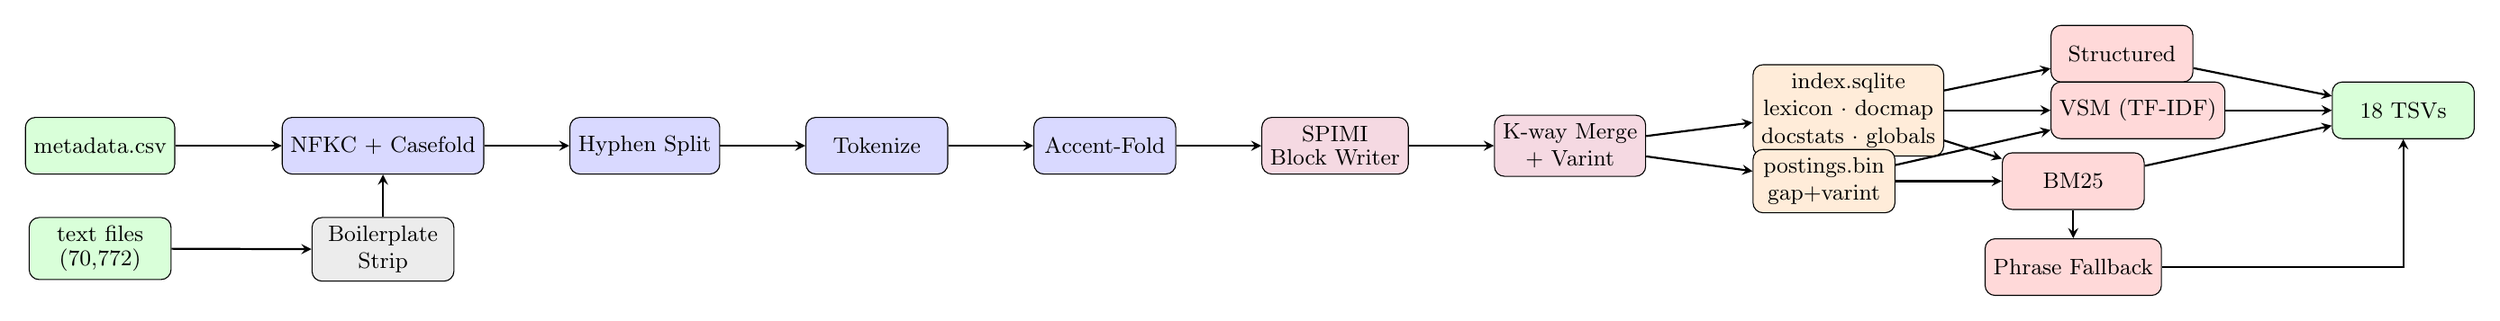
\begin{tikzpicture}[
    node distance=1.2cm and 1.5cm,
    box/.style={draw, rounded corners, minimum width=2cm, minimum height=0.8cm,
                fill=#1!15, font=\small},
    box/.default=blue,
    storage/.style={draw, minimum width=1.8cm, minimum height=0.8cm,
                    fill=orange!15, font=\small},
    arrow/.style={->, >=stealth, thick},
    label/.style={font=\footnotesize\itshape, text=gray}
]

% Input
\node[box=green] (csv) {metadata.csv};
\node[box=green, below=0.6cm of csv] (txt) {\shortstack{text files\\(70{,}772)}};

% Preprocessing
\node[box, right=1.5cm of csv] (nfkc) {NFKC + Casefold};
\node[box, right=1.2cm of nfkc] (hyph) {Hyphen Split};
\node[box, right=1.2cm of hyph] (tok) {Tokenize};
\node[box, right=1.2cm of tok] (alias) {Accent-Fold};
\node[box=gray, below=0.6cm of nfkc] (strip) {\shortstack{Boilerplate\\Strip}};

% Indexing
\node[box=purple, right=1.2cm of alias] (spimi) {\shortstack{SPIMI\\Block Writer}};
\node[box=purple, right=1.2cm of spimi] (merge) {\shortstack{K-way Merge\\+ Varint}};

% Storage
\node[box=orange, right=1.5cm of merge, yshift=0.5cm] (sqlite)
    {\shortstack{index.sqlite\\lexicon $\cdot$ docmap\\docstats $\cdot$ globals}};
\node[box=orange, right=1.5cm of merge, yshift=-0.5cm] (bin)
    {\shortstack{postings.bin\\gap+varint}};

% Retrieval
\node[box=red, right=1.5cm of sqlite, yshift=0.8cm] (struct) {Structured};
\node[box=red, right=1.5cm of sqlite, yshift=-0.0cm] (vsm) {VSM (TF-IDF)};
\node[box=red, right=1.5cm of bin, yshift=0.0cm] (bm25) {BM25};
\node[box=red, below=0.4cm of bm25] (phrase) {Phrase Fallback};

% Output
\node[box=green, right=1.5cm of vsm] (tsv) {18 TSVs};

% Arrows
\draw[arrow] (txt) -- (strip);
\draw[arrow] (strip) -- (nfkc);
\draw[arrow] (csv) -- (nfkc);
\draw[arrow] (nfkc) -- (hyph);
\draw[arrow] (hyph) -- (tok);
\draw[arrow] (tok) -- (alias);
\draw[arrow] (alias) -- (spimi);
\draw[arrow] (spimi) -- (merge);
\draw[arrow] (merge) -- (sqlite);
\draw[arrow] (merge) -- (bin);
\draw[arrow] (sqlite) -- (struct);
\draw[arrow] (sqlite) -- (vsm);
\draw[arrow] (sqlite) -- (bm25);
\draw[arrow] (bin) -- (vsm);
\draw[arrow] (bin) -- (bm25);
\draw[arrow] (bm25) -- (phrase);
\draw[arrow] (struct) -- (tsv);
\draw[arrow] (vsm) -- (tsv);
\draw[arrow] (bm25) -- (tsv);
\draw[arrow] (phrase) -| (tsv);

\end{tikzpicture}%
}
\caption{System architecture: data flows from raw text files through preprocessing and SPIMI indexing into a dual-store index (SQLite + binary postings), which serves three retrieval models producing ranked TSV outputs.}
\label{fig:architecture}
\end{figure*}

\begin{figure*}[t]
\centering
\resizebox{\textwidth}{!}{%
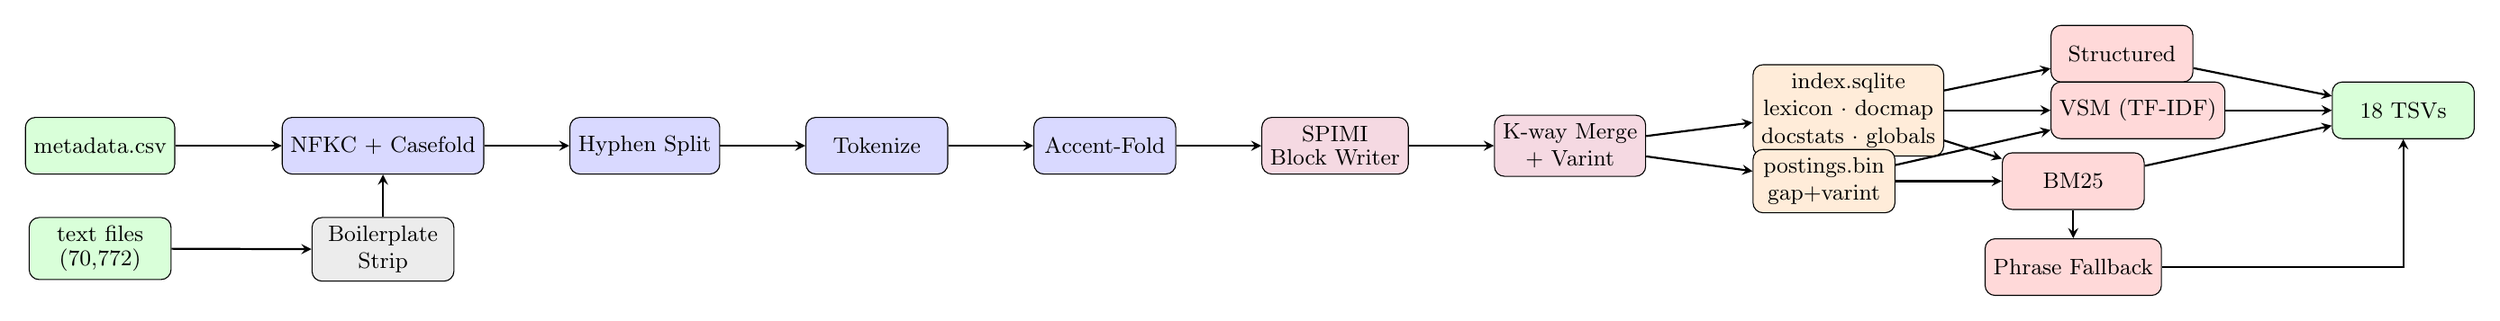
\begin{tikzpicture}[
    node distance=1.2cm and 1.5cm,
    box/.style={draw, rounded corners, minimum width=2cm, minimum height=0.8cm,
                fill=#1!15, font=\small},
    box/.default=blue,
    storage/.style={draw, minimum width=1.8cm, minimum height=0.8cm,
                    fill=orange!15, font=\small},
    arrow/.style={->, >=stealth, thick},
    label/.style={font=\footnotesize\itshape, text=gray}
]

% Input
\node[box=green] (csv) {metadata.csv};
\node[box=green, below=0.6cm of csv] (txt) {\shortstack{text files\\(70{,}772)}};

% Preprocessing
\node[box, right=1.5cm of csv] (nfkc) {NFKC + Casefold};
\node[box, right=1.2cm of nfkc] (hyph) {Hyphen Split};
\node[box, right=1.2cm of hyph] (tok) {Tokenize};
\node[box, right=1.2cm of tok] (alias) {Accent-Fold};
\node[box=gray, below=0.6cm of nfkc] (strip) {\shortstack{Boilerplate\\Strip}};

% Indexing
\node[box=purple, right=1.2cm of alias] (spimi) {\shortstack{SPIMI\\Block Writer}};
\node[box=purple, right=1.2cm of spimi] (merge) {\shortstack{K-way Merge\\+ Varint}};

% Storage
\node[box=orange, right=1.5cm of merge, yshift=0.5cm] (sqlite)
    {\shortstack{index.sqlite\\lexicon $\cdot$ docmap\\docstats $\cdot$ globals}};
\node[box=orange, right=1.5cm of merge, yshift=-0.5cm] (bin)
    {\shortstack{postings.bin\\gap+varint}};

% Retrieval
\node[box=red, right=1.5cm of sqlite, yshift=0.8cm] (struct) {Structured};
\node[box=red, right=1.5cm of sqlite, yshift=-0.0cm] (vsm) {VSM (TF-IDF)};
\node[box=red, right=1.5cm of bin, yshift=0.0cm] (bm25) {BM25};
\node[box=red, below=0.4cm of bm25] (phrase) {Phrase Fallback};

% Output
\node[box=green, right=1.5cm of vsm] (tsv) {18 TSVs};

% Arrows
\draw[arrow] (txt) -- (strip);
\draw[arrow] (strip) -- (nfkc);
\draw[arrow] (csv) -- (nfkc);
\draw[arrow] (nfkc) -- (hyph);
\draw[arrow] (hyph) -- (tok);
\draw[arrow] (tok) -- (alias);
\draw[arrow] (alias) -- (spimi);
\draw[arrow] (spimi) -- (merge);
\draw[arrow] (merge) -- (sqlite);
\draw[arrow] (merge) -- (bin);
\draw[arrow] (sqlite) -- (struct);
\draw[arrow] (sqlite) -- (vsm);
\draw[arrow] (sqlite) -- (bm25);
\draw[arrow] (bin) -- (vsm);
\draw[arrow] (bin) -- (bm25);
\draw[arrow] (bm25) -- (phrase);
\draw[arrow] (struct) -- (tsv);
\draw[arrow] (vsm) -- (tsv);
\draw[arrow] (bm25) -- (tsv);
\draw[arrow] (phrase) -| (tsv);

\end{tikzpicture}%
}
\caption{System architecture: data flows from raw text files through preprocessing and SPIMI indexing into a dual-store index (SQLite + binary postings), which serves three retrieval models producing ranked TSV outputs.}
\label{fig:architecture}
\end{figure*}


The system follows a standard IR pipeline (Figure~\ref{fig:architecture}):
raw text files and metadata are preprocessed, indexed into an inverted index
stored as a SQLite database plus a binary postings file, and searched via three
independent retrieval models.  All output is written as tab-separated value
(TSV) files in a deterministic, reproducible format.

\subsection{Preprocessing}
Text normalization follows a strict six-step pipeline applied identically to
both documents and queries:
\begin{enumerate}[nosep]
  \item \textbf{NFKC normalization}: Unicode compatibility decomposition
        followed by canonical composition.
  \item \textbf{Case folding}: Python's \texttt{str.casefold()} for
        locale-independent lowering (e.g., German ``\ss'' handled correctly).
  \item \textbf{Hyphen splitting}: Six Unicode dash variants (U+002D,
        U+2010 through U+2014) are replaced with spaces, splitting compound
        words into separate tokens.
  \item \textbf{Apostrophe removal}: U+0027 and U+2019 are deleted
        (``don't'' becomes ``dont'').
  \item \textbf{Tokenization}: The regex pattern
        \verb|[^\W_]+| extracts Unicode word tokens (letters and
        digits, excluding underscores).
  \item \textbf{Accent-fold aliases}: For both documents and queries,
        each token is NFD-decomposed and diacritical marks (Unicode
        category \texttt{Mn}) are stripped; if the result differs, both
        forms are indexed (e.g., ``dornr\"oschen'' generates both
        ``dornr\"oschen'' and ``dornroschen'').  Aliases do not
        contribute to document length.
\end{enumerate}

\paragraph{Design decisions.}
I deliberately chose \textbf{no stemming} and \textbf{no stopword removal}.
Implementing a correct multilingual stemmer risks harming proper nouns central
to the evaluation queries (e.g., ``Dick'' in Query~3, ``Dornr\"oschen'' in
Query~6).  For stopword removal, IDF weighting naturally suppresses
high-frequency terms; a global stopword list would break stopword-heavy queries
like ``to be, or not to be'' in the evaluation set.

\paragraph{Boilerplate stripping.}
Project Gutenberg headers and footers are stripped using
\texttt{*** START OF} / \texttt{*** END OF} markers (case-insensitive regex).
If a document contains both markers, all text outside that range is discarded.
If only one marker is found, the appropriate half is removed.  If neither
marker is found (some older Gutenberg files use non-standard formats), the
full text is indexed as a safe fallback.

% ============================================================
\section{Indexing}

The 27.8\,GB corpus far exceeds the 16\,GB RAM of the target machine,
making in-memory indexing impossible.  I use SPIMI~\cite{heinz2003spimi} to
partition the work into bounded memory blocks.

\subsection{SPIMI Block Building}
This subsection describes how documents are ingested into memory-bounded
blocks and flushed to disk.
Documents are processed sequentially in sorted \texttt{gutenberg\_id} order
(for deterministic document-ID assignment).  For each document, the
preprocessed tokens are counted into a term-frequency map, and each
(term, docid, tf) triple is appended to the in-memory inverted index.
Accent-fold aliases are indexed with the same tf value as their base tokens but
do not inflate the document length counter.

\paragraph{Dual flush thresholds.}
The in-memory block is flushed to disk when \emph{either} of two conditions is
met:
\begin{itemize}[nosep]
  \item \texttt{tracemalloc} current allocation $\geq$ 350\,MB, or
  \item Unique term count in the current block $\geq$ 1{,}000{,}000.
\end{itemize}
Both thresholds are checked after every document.  Using \texttt{tracemalloc}
rather than RSS monitoring is a deliberate choice: it measures only
Python-allocated objects, providing a consistent and portable metric.  However,
actual RSS during indexing can be 1.5--2$\times$ higher than the traced value
due to Python's memory allocator overhead and the C-level buffers used by
SQLite and file I/O.  For the full corpus, the SPIMI phase produced 150 blocks
totalling 4.5\,GB on disk.

\paragraph{Block flush procedure.}
Each flush sorts the in-memory terms lexicographically, sorts each
term's postings by document-ID, and writes them to a block-specific
binary file using varint encoding.  A companion JSON lexicon maps each
term to its (df, offset, length) triple within the block postings file.
After flushing, the in-memory dictionary is cleared,
\texttt{gc.collect()} is called, and the \texttt{tracemalloc} trace
buffer is reset.

\subsection{Handling 27.8\,GB on 16\,GB RAM}
Fitting the full build into limited memory required four complementary strategies.
The most challenging engineering aspect of this project was making the full
corpus index build survive on a machine with only 16\,GB of physical RAM.
Several strategies contributed to this:
\begin{itemize}[nosep]
  \item \textbf{Aggressive garbage collection.}  After every block flush, I
        call \texttt{gc.collect()} and reset the \texttt{tracemalloc} trace
        buffer to prevent monotonic memory growth.
  \item \textbf{Single-pass file reads.}  Each document is read, preprocessed,
        and discarded before the next is opened.
  \item \textbf{Memory-aware merge.}  All 150 block lexicons are explicitly
        deleted before the doc\_norm pass begins, preventing overlap.
  \item \textbf{Block cleanup.}  The 4.5\,GB \texttt{blocks/} directory is
        removed via \texttt{shutil.rmtree()} after a successful merge.
\end{itemize}
Despite these measures, loading all 150 block lexicons simultaneously caused
significant swap thrashing, stretching the merge phase to approximately 8 hours
versus 2.5 hours for block building.

\subsection{K-way Merge}
The merge phase consolidates 150 blocks into one compressed postings file and
precomputes the statistics needed at query time.
After all blocks are flushed, a K-way merge consolidates them into the final
index.  All 150 block postings files are opened simultaneously, and the
block lexicons are loaded into memory.  Terms are iterated in global
lexicographic order; for each term, posting lists from all contributing blocks
are concatenated, sorted by document-ID, delta-encoded (gap compression), and
written using variable-length byte encoding (varint).  This reduces the
postings file from 4.5\,GB (raw blocks) to 1.15\,GB (compressed), a 75\%
reduction.

The merge also precomputes per-document statistics needed at query time:
\begin{itemize}[nosep]
  \item \textbf{Document lengths} ($|d|$): total tokens after preprocessing,
        stored in the \texttt{docstats} table.
  \item \textbf{VSM norms} ($\|d\|$): computed in a mandatory post-merge pass
        (Section~\ref{sec:docnorm}).
  \item \textbf{Global statistics}: $N = 70{,}772$ and
        $\text{avgdl} = 61{,}570$ tokens, stored in the \texttt{globals} table.
\end{itemize}

\subsection{doc\_norm Computation}\label{sec:docnorm}
Exact L2 norms are computed in a single post-merge pass so that VSM cosine
scores are correct at query time.
After the merge, I perform a single sequential pass over the entire postings
file to compute exact L2 norms for every document.  The lexicon is iterated in
\texttt{ORDER BY offset ASC} to guarantee sequential I/O.  For each term with
document frequency $\text{df}_t$, I compute:
\begin{equation}
  \text{idf}_t = \ln\!\left(\frac{N + 1}{\text{df}_t + 1}\right) + 1
\end{equation}
and for each (docid, tf) posting:
$w = (1 + \ln(\text{tf})) \cdot \text{idf}_t$; then
$\text{norm\_acc}[\text{docid}] \mathrel{+}= w^2$.
The final norm is $\|d\| = \sqrt{\text{norm\_acc}[\text{docid}]}$.  A defensive
guard (\texttt{if tf <= 0: continue}) prevents \texttt{math.log(0)}
domain errors from potentially corrupted postings.  Of the 70{,}772 indexed
documents,
65 have $\|d\| = 0$ because their text files yielded zero tokens after
boilerplate stripping (empty or binary-only files); these documents receive
no VSM score at query time since the cosine denominator is zero.

\subsection{Storage Format}

% Index Format Diagram (TikZ)
% Include with: % Index Format Diagram (TikZ)
% Include with: % Index Format Diagram (TikZ)
% Include with: \input{figures/index_format.tex}
\begin{figure}[t]
\centering
\resizebox{\columnwidth}{!}{%
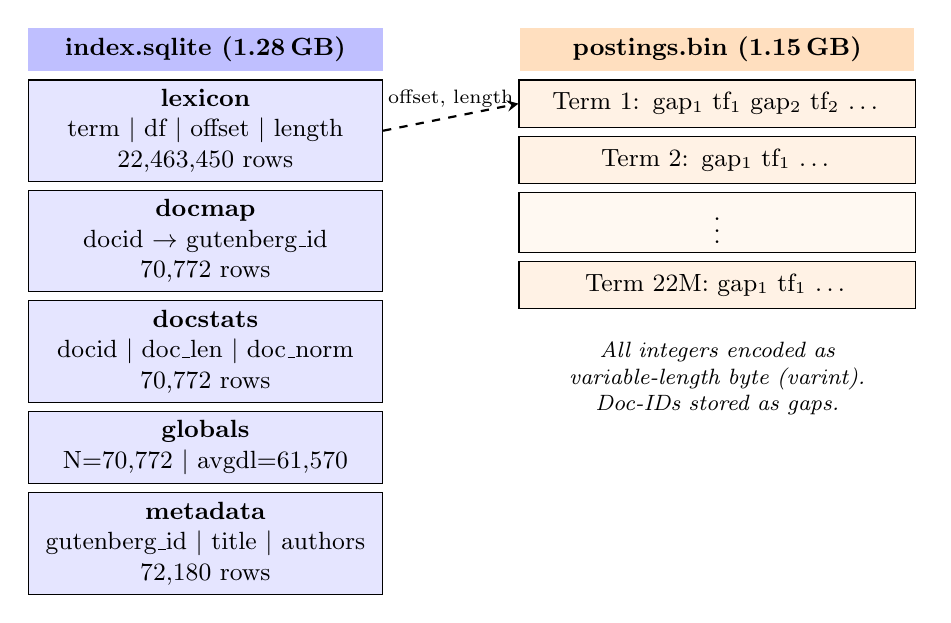
\begin{tikzpicture}[
    table/.style={draw, minimum width=4.5cm, minimum height=0.6cm,
                  fill=#1!10, font=\small, align=center},
    table/.default=blue,
    bintable/.style={draw, minimum width=4.5cm, minimum height=0.6cm,
                     fill=orange!10, font=\small, align=center},
    header/.style={font=\small\bfseries, fill=#1!25},
    header/.default=blue,
    arrow/.style={->, >=stealth, thick, dashed},
]

% SQLite column
\node[header, minimum width=4.5cm, minimum height=0.5cm] (sh) at (0,0)
    {index.sqlite (1.28\,GB)};

\node[table, below=0.1cm of sh] (lex)
    {\textbf{lexicon}\\term $|$ df $|$ offset $|$ length\\22{,}463{,}450 rows};
\node[table, below=0.1cm of lex] (dmap)
    {\textbf{docmap}\\docid $\to$ gutenberg\_id\\70{,}772 rows};
\node[table, below=0.1cm of dmap] (dstat)
    {\textbf{docstats}\\docid $|$ doc\_len $|$ doc\_norm\\70{,}772 rows};
\node[table, below=0.1cm of dstat] (glob)
    {\textbf{globals}\\N=70{,}772 $|$ avgdl=61{,}570};
\node[table, below=0.1cm of glob] (meta)
    {\textbf{metadata}\\gutenberg\_id $|$ title $|$ authors\\72{,}180 rows};

% Postings column
\node[header=orange, minimum width=5cm, minimum height=0.5cm]
    (ph) at (6.5,0) {postings.bin (1.15\,GB)};

\node[bintable, below=0.1cm of ph, text width=4.8cm] (p1)
    {Term 1: gap$_1$ tf$_1$ gap$_2$ tf$_2$ \ldots};
\node[bintable, below=0.1cm of p1, text width=4.8cm] (p2)
    {Term 2: gap$_1$ tf$_1$ \ldots};
\node[bintable, below=0.1cm of p2, text width=4.8cm, fill=orange!5] (dots)
    {\vdots};
\node[bintable, below=0.1cm of dots, text width=4.8cm] (pn)
    {Term 22M: gap$_1$ tf$_1$ \ldots};

% Encoding note
\node[below=0.3cm of pn, font=\footnotesize\itshape, text width=5cm, align=center]
    {All integers encoded as\\variable-length byte (varint).\\Doc-IDs stored as gaps.};

% Arrow from lexicon to postings
\draw[arrow] (lex.east) -- node[above, font=\scriptsize] {offset, length} (p1.west);

\end{tikzpicture}%
}
\caption{Index storage format: SQLite stores the lexicon (mapping terms to postings offsets), document maps, statistics, and metadata. The postings file uses varint-encoded gap compression for doc-IDs and term frequencies.}
\label{fig:index-format}
\end{figure}

\begin{figure}[t]
\centering
\resizebox{\columnwidth}{!}{%
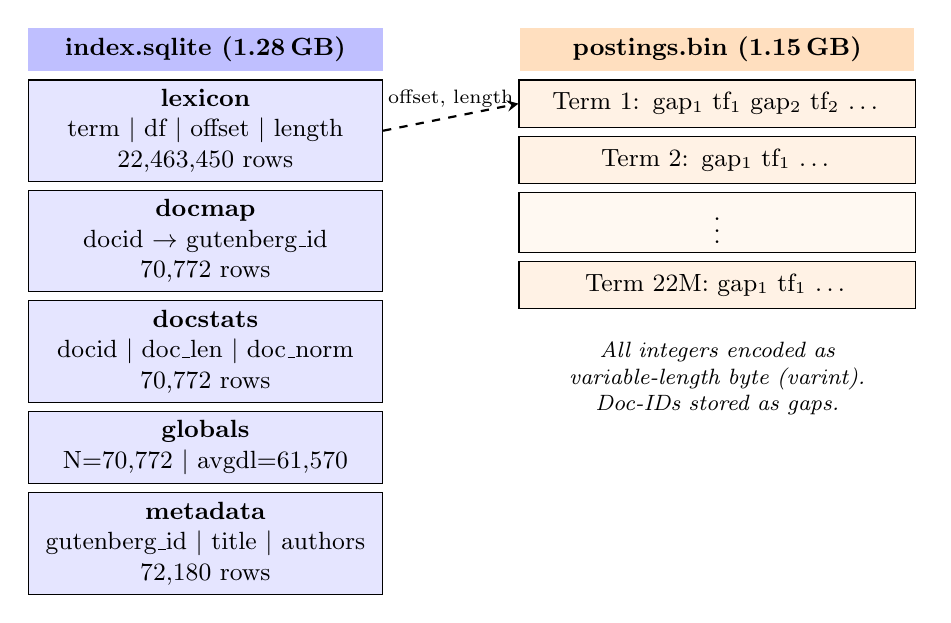
\begin{tikzpicture}[
    table/.style={draw, minimum width=4.5cm, minimum height=0.6cm,
                  fill=#1!10, font=\small, align=center},
    table/.default=blue,
    bintable/.style={draw, minimum width=4.5cm, minimum height=0.6cm,
                     fill=orange!10, font=\small, align=center},
    header/.style={font=\small\bfseries, fill=#1!25},
    header/.default=blue,
    arrow/.style={->, >=stealth, thick, dashed},
]

% SQLite column
\node[header, minimum width=4.5cm, minimum height=0.5cm] (sh) at (0,0)
    {index.sqlite (1.28\,GB)};

\node[table, below=0.1cm of sh] (lex)
    {\textbf{lexicon}\\term $|$ df $|$ offset $|$ length\\22{,}463{,}450 rows};
\node[table, below=0.1cm of lex] (dmap)
    {\textbf{docmap}\\docid $\to$ gutenberg\_id\\70{,}772 rows};
\node[table, below=0.1cm of dmap] (dstat)
    {\textbf{docstats}\\docid $|$ doc\_len $|$ doc\_norm\\70{,}772 rows};
\node[table, below=0.1cm of dstat] (glob)
    {\textbf{globals}\\N=70{,}772 $|$ avgdl=61{,}570};
\node[table, below=0.1cm of glob] (meta)
    {\textbf{metadata}\\gutenberg\_id $|$ title $|$ authors\\72{,}180 rows};

% Postings column
\node[header=orange, minimum width=5cm, minimum height=0.5cm]
    (ph) at (6.5,0) {postings.bin (1.15\,GB)};

\node[bintable, below=0.1cm of ph, text width=4.8cm] (p1)
    {Term 1: gap$_1$ tf$_1$ gap$_2$ tf$_2$ \ldots};
\node[bintable, below=0.1cm of p1, text width=4.8cm] (p2)
    {Term 2: gap$_1$ tf$_1$ \ldots};
\node[bintable, below=0.1cm of p2, text width=4.8cm, fill=orange!5] (dots)
    {\vdots};
\node[bintable, below=0.1cm of dots, text width=4.8cm] (pn)
    {Term 22M: gap$_1$ tf$_1$ \ldots};

% Encoding note
\node[below=0.3cm of pn, font=\footnotesize\itshape, text width=5cm, align=center]
    {All integers encoded as\\variable-length byte (varint).\\Doc-IDs stored as gaps.};

% Arrow from lexicon to postings
\draw[arrow] (lex.east) -- node[above, font=\scriptsize] {offset, length} (p1.west);

\end{tikzpicture}%
}
\caption{Index storage format: SQLite stores the lexicon (mapping terms to postings offsets), document maps, statistics, and metadata. The postings file uses varint-encoded gap compression for doc-IDs and term frequencies.}
\label{fig:index-format}
\end{figure}

\begin{figure}[t]
\centering
\resizebox{\columnwidth}{!}{%
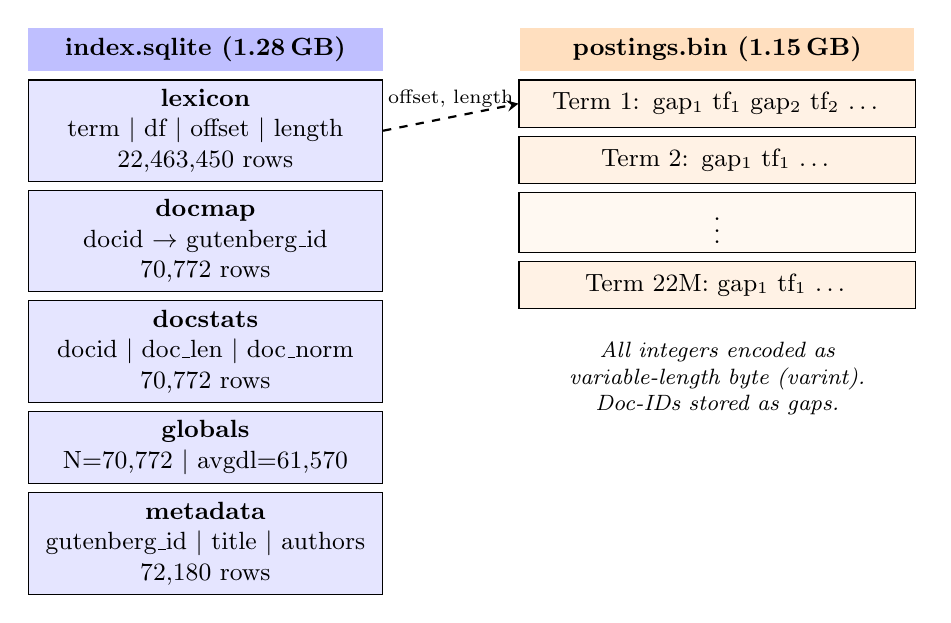
\begin{tikzpicture}[
    table/.style={draw, minimum width=4.5cm, minimum height=0.6cm,
                  fill=#1!10, font=\small, align=center},
    table/.default=blue,
    bintable/.style={draw, minimum width=4.5cm, minimum height=0.6cm,
                     fill=orange!10, font=\small, align=center},
    header/.style={font=\small\bfseries, fill=#1!25},
    header/.default=blue,
    arrow/.style={->, >=stealth, thick, dashed},
]

% SQLite column
\node[header, minimum width=4.5cm, minimum height=0.5cm] (sh) at (0,0)
    {index.sqlite (1.28\,GB)};

\node[table, below=0.1cm of sh] (lex)
    {\textbf{lexicon}\\term $|$ df $|$ offset $|$ length\\22{,}463{,}450 rows};
\node[table, below=0.1cm of lex] (dmap)
    {\textbf{docmap}\\docid $\to$ gutenberg\_id\\70{,}772 rows};
\node[table, below=0.1cm of dmap] (dstat)
    {\textbf{docstats}\\docid $|$ doc\_len $|$ doc\_norm\\70{,}772 rows};
\node[table, below=0.1cm of dstat] (glob)
    {\textbf{globals}\\N=70{,}772 $|$ avgdl=61{,}570};
\node[table, below=0.1cm of glob] (meta)
    {\textbf{metadata}\\gutenberg\_id $|$ title $|$ authors\\72{,}180 rows};

% Postings column
\node[header=orange, minimum width=5cm, minimum height=0.5cm]
    (ph) at (6.5,0) {postings.bin (1.15\,GB)};

\node[bintable, below=0.1cm of ph, text width=4.8cm] (p1)
    {Term 1: gap$_1$ tf$_1$ gap$_2$ tf$_2$ \ldots};
\node[bintable, below=0.1cm of p1, text width=4.8cm] (p2)
    {Term 2: gap$_1$ tf$_1$ \ldots};
\node[bintable, below=0.1cm of p2, text width=4.8cm, fill=orange!5] (dots)
    {\vdots};
\node[bintable, below=0.1cm of dots, text width=4.8cm] (pn)
    {Term 22M: gap$_1$ tf$_1$ \ldots};

% Encoding note
\node[below=0.3cm of pn, font=\footnotesize\itshape, text width=5cm, align=center]
    {All integers encoded as\\variable-length byte (varint).\\Doc-IDs stored as gaps.};

% Arrow from lexicon to postings
\draw[arrow] (lex.east) -- node[above, font=\scriptsize] {offset, length} (p1.west);

\end{tikzpicture}%
}
\caption{Index storage format: SQLite stores the lexicon (mapping terms to postings offsets), document maps, statistics, and metadata. The postings file uses varint-encoded gap compression for doc-IDs and term frequencies.}
\label{fig:index-format}
\end{figure}


The final index consists of two files (Figure~\ref{fig:index-format}):
\begin{itemize}[nosep]
  \item \textbf{index.sqlite} (1.28\,GB): Contains the \texttt{lexicon} table
        (term $\to$ df, byte offset, byte length), \texttt{docmap}
        (\texttt{docid} $\to$ \texttt{gutenberg\_id}), \texttt{docstats} (document lengths and
        L2 norms), \texttt{globals} ($N$, avgdl, build parameters), and
        \texttt{metadata} (titles, authors, bookshelves for 72{,}180 rows
        including entries without text files).
  \item \textbf{postings.bin} (1.15\,GB): A flat binary file of varint-encoded
        posting lists, accessed via (offset, length) pairs from the lexicon.
        Each posting list stores a varint-encoded df, followed by df pairs of
        (gap, tf) varints.
\end{itemize}

% ============================================================
\section{Ranking Models}

\subsection{Structured Metadata Search}
The structured model searches only the \texttt{metadata} table (title, authors,
language, bookshelf, rights), applying a heuristic scoring formula:
\begin{equation}
  \text{score}(q, d) = 10 \cdot f_{\text{title}} + 5 \cdot f_{\text{author}}
                      + 2 \cdot h_{\text{title}} + h_{\text{author}} + h_{\text{other}}
\end{equation}
where $f_{\text{title}} = 1$ if the normalized query is a substring of the
normalized title (else 0); $f_{\text{author}} = 1$ if the query matches an
author via token-sorted comparison (to handle Gutenberg's ``Last, First''
name format); and $h_{\text{title}}$, $h_{\text{author}}$, $h_{\text{other}}$
count distinct query tokens found in each field.

The token-sorted author comparison deserves explanation: Gutenberg stores names
as ``Dick, Philip K.'' which normalizes to ``dick philip k''.  By sorting both
the query tokens and the author tokens alphabetically before comparison, I
correctly identify ``philip k dick'' as matching ``dick philip k'' regardless of
name order.  Without this fix, the author-exact bonus would never fire for
real Gutenberg queries.

This model represents a \textbf{fundamentally different retrieval mechanism}
from VSM and BM25: field-weighted heuristic matching versus vector-space
geometric similarity versus probabilistic term weighting.  The three-way
comparison is central to the evaluation.

\subsection{Vector Space Model (VSM)}
The VSM implements TF-IDF cosine similarity~\cite{salton1975vsm}.  For each
query term $t$ with query frequency $\text{tf}_{t,q}$:
\begin{equation}
  w_{t,q} = (1 + \ln(\text{tf}_{t,q})) \cdot \text{idf}_t, \quad
  w_{t,d} = (1 + \ln(\text{tf}_{t,d})) \cdot \text{idf}_t
\end{equation}
where $\text{idf}_t = \ln\!\bigl(\frac{N+1}{\text{df}_t+1}\bigr) + 1$ (the
smoothed, always-positive variant).  The cosine similarity is:
\begin{equation}
  \text{score}(q, d) = \frac{\sum_{t \in q} w_{t,q} \cdot w_{t,d}}
                             {\|q\| \cdot \|d\|}
\end{equation}
The query norm $\|q\|$ is computed at query time from the $w_{t,q}$ values; the
document norm $\|d\|$ is precomputed during indexing and loaded at startup for
O(1) lookup.  The IDF is computed once per query term, outside the postings
loop, and the same \texttt{idf\_t} variable is reused for both $w_{t,q}$ and
$w_{t,d}$.  This avoids any redundant lexicon lookups inside the inner loop.

\paragraph{Stopword-heavy early-abort.}
When more than 60\% of query tokens have $\text{df}_t / N > 0.8$ (or the query
contains quoted phrases), VSM returns an \textbf{empty result set} immediately.
This is not a bug but a theoretically motivated design decision: when all query
tokens are near-stopwords, their IDF values are near-identical, producing
near-tied scores across most of the corpus with no discriminative value.  Rather
than computing and returning a ranking that is effectively random, the system
aborts early.  This behaviour is a key finding in the evaluation (Section~\ref{sec:eval}).

\subsection{BM25}
I implement Okapi BM25~\cite{robertson1994okapi,robertson2009bm25} with
parameters $k_1 = 1.2$ and $b = 0.75$:
\begin{equation}
  \text{score}(q, d) = \sum_{t \in q} \text{IDF}(t) \cdot
  \frac{\text{tf}_{t,d} \cdot (k_1 + 1)}
       {\text{tf}_{t,d} + k_1 \cdot \bigl(1 - b + b \cdot \frac{|d|}{\text{avgdl}}\bigr)}
\end{equation}
where $\text{IDF}(t) = \ln\!\bigl(\frac{N - \text{df}_t + 0.5}{\text{df}_t + 0.5}\bigr)$.
Terms with $\text{IDF} \leq 0$ or $\text{df}_t / N > 0.8$ are skipped entirely,
and their posting lists are never decoded.  This is both a correctness measure
(negative IDF would reduce scores) and a performance optimization (high-df
terms have massive posting lists).

\paragraph{Parameter justification.}
The values $k_1 = 1.2$ and $b = 0.75$ are the standard defaults established by
Robertson and Walker~\cite{robertson1994okapi} and empirically validated on TREC
collections~\cite{robertson1995trec3}.  For the Gutenberg corpus, where
documents range from short poems to 900{,}000-token compilations, the standard
$b = 0.75$ provides effective length normalization without over-penalizing long
documents.  The TF saturation at $k_1 = 1.2$ prevents high raw term
frequencies (common in full-length books) from dominating the score.

\subsection{Phrase Fallback}
When the phrase-fallback trigger fires (quoted phrases or $>$60\% high-df
tokens) and BM25 returns zero candidates (because all terms have zero IDF),
the system performs a full-corpus substring scan:
\begin{enumerate}[nosep]
  \item Normalize the query phrase: NFKC, casefold, replace \emph{all}
        non-alphanumeric characters with spaces, collapse whitespace.
  \item Iterate through every text file in sorted order.
  \item For each file, apply the same normalization and check for the phrase
        as a substring.
  \item Award a fixed boost score of 5.0 to matches.
  \item Cap at 200 matches for practical runtime bounds.
\end{enumerate}
If BM25 does return candidates (partial IDF signal), the phrase check is
applied as a boost: matching candidates receive $+5.0$ added to their BM25
score and results are re-sorted.

This mechanism is a pragmatic compromise.  The Q1 full-corpus scan takes
approximately 459 seconds (compared to sub-100\,ms for normal queries),
highlighting the need for positional inverted indices in future work.

% ============================================================
\section{Implementation Details}

\subsection{Startup Loading}
Before any query is processed, five structures are loaded into memory from
SQLite in a single JOIN query:
\begin{itemize}[nosep]
  \item \texttt{docid\_to\_gutid}: maps internal \texttt{docid} to Gutenberg~ID
        (for sorting results).
  \item \texttt{doc\_len}: maps \texttt{docid} to token count (for BM25 denominator).
  \item \texttt{doc\_norm}: maps \texttt{docid} to L2 norm (for VSM cosine divisor).
  \item $N$: total indexed documents (70{,}772).
  \item \texttt{avgdl}: average document length (61{,}570 tokens).
\end{itemize}
All five fit in approximately 3.5\,MB of RAM ($\sim$70{,}000 entries $\times$
$\sim$50 bytes each).  Crucially, \texttt{doc\_len} and \texttt{doc\_norm} are
accessed inside the innermost scoring loops (once per posting per query term),
so O(1) dict lookups are essential.  A SQLite lookup in the inner loop would
make every query take minutes instead of milliseconds.

\subsection{Postings Cache}
A session-scoped cache keyed by (offset, length) avoids redundant postings
decoding when the same term appears across queries within a single process run.

\subsection{Determinism}
Reproducible output is guaranteed by: (1)~document ID assignment by sorted
Gutenberg ID order, (2)~scores rounded to 6 decimal places before sorting
(accepting a negligible ranking perturbation in exchange for deterministic
output), and (3)~tie-breaking by lexicographic Gutenberg ID (ascending).
Combined with the fixed preprocessing pipeline, every run produces
byte-identical TSV files.

\subsection{Snippet Generation}
For each result, a 250-character snippet is generated by: (a)~selecting the
query token with the highest \emph{VSM} IDF (the smoothed formula is always
positive, unlike BM25 IDF which can be zero for high-frequency terms);
(b)~finding its first character-level occurrence in the raw document text;
(c)~extracting a 250-character window centred on the match; (d)~collapsing
internal whitespace.  The \texttt{start\_line} is computed as
$1 + \text{count of newlines before the snippet start position}$.

\subsection{Metadata Handling}
The Gutenberg metadata CSV contains 75{,}473 rows with duplicates (multi-author
entries for the same book).  I deduplicate by grouping on \texttt{gutenberg\_id},
merging author fields with semicolon-separated unique values in sorted order.
A \texttt{has\_text} flag marks whether the corresponding text file exists;
1{,}408 IDs in the metadata lack text files.  These are retained in the
metadata table for structured search but excluded from the full-text index.

\subsection{Interactive Query Interface}
Beyond the batch evaluation runner, the system provides an interactive
REPL invoked via \texttt{python -m ir\_system interactive}.  The user
selects a model (structured, VSM, or BM25), enters a free-text query,
and optionally sets the number of results (default~10).  Each result is
displayed with its rank, Gutenberg ID, score, title, authors, and an empty
snippet field (reserved for future enhancement).  This
interface enables exploratory search beyond the fixed evaluation set.

% ============================================================
\section{Evaluation}\label{sec:eval}

I evaluate the system using six queries specified in the assignment
(Table~\ref{tab:queries}), deliberately chosen to exercise different retrieval
scenarios: metadata matching (Q2, Q3), content retrieval (Q4), stopword-heavy
phrasing (Q1), boilerplate-confounded terms (Q5), and multilingual Unicode (Q6).

\begin{table}[h]
\centering
\caption{Evaluation Queries}
\label{tab:queries}
\begin{tabular}{cl}
\toprule
Q\# & Query Text \\
\midrule
1 & to be, or not to be \\
2 & English Grammar \\
3 & Philip K Dick \\
4 & Jabberwocky \\
5 & Gutenberg \\
6 & Dornr\"oschen \\
\bottomrule
\end{tabular}
\end{table}

\subsection{Methodology}
Each query is executed against all three models, producing up to 100 ranked
results per query-model pair in five-column TSV files (rank, Gutenberg ID,
score, snippet, start\_line) as required by the assignment specification;
18~TSV files are included in the repository.
For each query$\times$model combination (18 total; 3 TSVs are empty due to
design-intentional early-abort or missing metadata matches), I manually judged
the top-10 results using a three-point relevance scale: 1$=$relevant,
2$=$partially relevant, 0$=$not relevant.  This produced 150 judgment labels
across 15 non-empty result sets.

I compute four metrics:
\begin{itemize}[nosep]
  \item \textbf{P@10}: Precision at 10 (partial counted as 0).
  \item \textbf{P@10\textsubscript{p}}: Precision at 10 (partial counted as 0.5).
  \item \textbf{AP@10}: Average Precision over the judged top-10.
  \item \textbf{NDCG@10}: Gain values: relevant$=$1.0, partial$=$0.5,
        not relevant$=$0.0.
\end{itemize}

\textbf{Limitations.}  Metrics are computed over only the retrieved top-10; no
exhaustive relevance judgments (qrels) exist for the full corpus.  With six
queries and a single annotator, the results should be interpreted as case-study
observations rather than statistically significant conclusions.  A different
query set could rank the models differently; in particular, queries requiring
entity resolution or cross-lingual matching remain untested.

\subsection{Results}

\begin{table*}[t]
\centering
\caption{Evaluation Metrics per Query and Model (top-10 judged)}
\label{tab:eval-metrics}
\begin{tabular}{clccccc}
\toprule
Q\# & Model & P@10 & P@10\textsubscript{p} & AP@10 & NDCG@10 & \#Results \\
\midrule
1 & bm25 & 0.2000 & 0.4500 & 0.7500 & 0.8916 & 10 \\
1 & structured & 0.0000 & 0.0000 & 0.0000 & 0.0000 & 10 \\
\midrule
2 & bm25 & 0.2000 & 0.4500 & 0.1944 & 0.6523 & 10 \\
2 & structured & 1.0000 & 1.0000 & 1.0000 & 1.0000 & 10 \\
2 & vsm & 0.2000 & 0.3000 & 0.3611 & 0.5993 & 10 \\
\midrule
3 & bm25 & 0.0000 & 0.0000 & 0.0000 & 0.0000 & 10 \\
3 & structured & 1.0000 & 1.0000 & 1.0000 & 1.0000 & 10 \\
3 & vsm & 0.2000 & 0.2000 & 0.3750 & 0.5803 & 10 \\
\midrule
4 & bm25 & 0.6000 & 0.8000 & 0.9762 & 0.9971 & 10 \\
4 & vsm & 0.7000 & 0.8500 & 0.9094 & 0.9859 & 10 \\
\midrule
5 & bm25 & 0.4000 & 0.5000 & 0.4512 & 0.7813 & 10 \\
5 & structured & 0.1000 & 0.5500 & 1.0000 & 1.0000 & 10 \\
5 & vsm & 0.0000 & 0.2500 & 0.0000 & 0.8753 & 10 \\
\midrule
6 & bm25 & 0.2000 & 0.5000 & 0.2667 & 0.8352 & 10 \\
6 & vsm & 0.1000 & 0.4500 & 0.1429 & 0.8345 & 10 \\
\bottomrule
\end{tabular}
\end{table*}


Table~\ref{tab:eval-metrics} shows per-query results.  I discuss each query in
turn, tying the observations back to model design choices.

\paragraph{Q1 (``to be, or not to be'').}
All six tokens are common English stopwords.  \textbf{Structured} matched title
fragments irrelevantly (P@10$=$0); titles like ``How Not to Be Them'' contain
the words but have no connection to Shakespeare.  \textbf{VSM} correctly
early-aborted (zero results), detecting that all tokens have df/N~$>$~0.8 and
would produce near-tied scores with no discriminative signal.  This is exactly
the behaviour predicted by IDF theory: when every term occurs in most documents,
cosine similarity degenerates to near-uniform scores.  \textbf{BM25}'s phrase
fallback activated a full-corpus scan, finding Shakespeare's Complete Works at
rank~1 (P@10$=$0.20, NDCG$=$0.89).  Literary biographies and criticism that
quote the phrase scored as partially relevant.

\paragraph{Q2 (``English Grammar'').}
\textbf{Structured} achieved perfect precision (P@10$=$1.0): all 10 results
are actual English grammar textbooks, matched by title-field substring matching.
\textbf{BM25} and \textbf{VSM} both returned P@10$=$0.20, because fiction set
in ``grammar schools'' and short catalog entries where ``grammar'' appears with
high frequency ranked above the actual textbooks.  This illustrates that
bag-of-words models cannot distinguish between topic-relevant uses and
incidental mentions of query terms.

\paragraph{Q3 (``Philip K Dick'').}
\textbf{Structured} again achieved P@10$=$1.0 via token-sorted
author-field matching (``Dick, Philip K.'' in Gutenberg metadata).
\textbf{BM25} failed completely (P@10$=$0.0): the token ``Dick''
overwhelmingly matches dime novels, copyright catalogs, and motion
picture credits, while ``Philip'' and ``K'' provide weak discriminative
power.  This is the most striking demonstration of the bag-of-words
limitation for multi-word proper nouns.  \textbf{VSM} managed
P@10$=$0.20, finding two actual PKD stories through higher IDF for
``philip'' in combination with ``dick''.

\paragraph{Q4 (``Jabberwocky'').}
Both \textbf{BM25} (P@10$=$0.60) and \textbf{VSM} (P@10$=$0.70) performed
strongly, since ``Jabberwocky'' is a highly distinctive single term with
excellent IDF.  The top-10 lists overlap substantially (Jaccard$=$0.82),
confirming that both models correctly identify the same informative term.
\textbf{Structured} returned empty results because ``Jabberwocky'' is a poem
title within ``Through the Looking-Glass'', not a standalone book title in the
metadata.

\paragraph{Q5 (``Gutenberg'').}
Results are confounded by the ``Project Gutenberg'' boilerplate.  Although
I strip headers, some non-standard files retain header fragments.
\textbf{BM25} achieved P@10$=$0.40, finding a French play about Johannes
Gutenberg the inventor and several Project Gutenberg history documents.
\textbf{Structured} (P@10$=$0.10) returned mostly PG index compilations with
``Gutenberg'' in the title.  \textbf{VSM} (P@10$=$0.00) is most vulnerable to
the boilerplate issue: very short documents where a single residual
``Gutenberg'' mention gives a disproportionately high TF-IDF score.

\paragraph{Q6 (``Dornr\"oschen'').}
\textbf{BM25} found German fairy tale collections (P@10$=$0.20,
NDCG$=$0.84), including Bechstein's M\"archenbuch and
G\"ansem\"utterchens M\"archen.  The accent-fold aliasing was
critical here: the query generates both ``dornr\"oschen'' and
``dornroschen'', matching documents regardless of whether they use the
diacritic form.  \textbf{VSM} produced similar results (P@10$=$0.10,
Jaccard$=$0.67 with BM25).  \textbf{Structured} returned empty results because
German fairy tales are catalogued under collection titles, not individual tale
names.

\subsection{Model Comparison}

\begin{table}[h]
\centering
\caption{Top-10 Overlap (Jaccard) Between Models}
\label{tab:overlap}
\begin{tabular}{clcc}
\toprule
Q\# & Model Pair & Overlap & Jaccard \\
\midrule
1 & structured vs vsm & 0 & 0.0000 \\
1 & structured vs bm25 & 0 & 0.0000 \\
1 & vsm vs bm25 & 0 & 0.0000 \\
\midrule
2 & structured vs vsm & 1 & 0.0526 \\
2 & structured vs bm25 & 1 & 0.0526 \\
2 & vsm vs bm25 & 0 & 0.0000 \\
\midrule
3 & structured vs vsm & 2 & 0.1111 \\
3 & structured vs bm25 & 0 & 0.0000 \\
3 & vsm vs bm25 & 0 & 0.0000 \\
\midrule
4 & structured vs vsm & 0 & 0.0000 \\
4 & structured vs bm25 & 0 & 0.0000 \\
4 & vsm vs bm25 & 9 & 0.8182 \\
\midrule
5 & structured vs vsm & 0 & 0.0000 \\
5 & structured vs bm25 & 0 & 0.0000 \\
5 & vsm vs bm25 & 0 & 0.0000 \\
\midrule
6 & structured vs vsm & 0 & 0.0000 \\
6 & structured vs bm25 & 0 & 0.0000 \\
6 & vsm vs bm25 & 8 & 0.6667 \\
\bottomrule
\end{tabular}
\end{table}


Table~\ref{tab:overlap} shows pairwise top-10 overlap between models.  Three
patterns emerge clearly:
\begin{enumerate}[nosep]
  \item \textbf{Structured vs.\ full-text models have near-zero overlap.}
        They address fundamentally different query types and should be seen
        as complementary, not competing, retrieval strategies.
  \item \textbf{VSM and BM25 converge for distinctive terms} (Q4:
        Jaccard$=$0.82; Q6: 0.67) but diverge for common terms where BM25's
        length normalization makes a difference.
  \item \textbf{BM25 outperforms VSM on aggregate metrics}
        (mean AP@10: 0.44 vs.\ 0.36), primarily because the
        $|d|/\text{avgdl}$ factor in BM25 penalizes very long documents and
        prevents the short-document bias that TF-IDF cosine similarity exhibits.
\end{enumerate}

\subsection{Aggregate Performance}

\begin{table}[h]
\centering
\caption{Mean Evaluation Metrics per Model}
\label{tab:model-summary}
\begin{tabular}{lcccc}
\toprule
Model & P@10 & P@10\textsubscript{p} & AP@10 & NDCG@10 \\
\midrule
Structured & 0.525 & 0.638 & 0.750 & 0.750 \\
VSM        & 0.240 & 0.410 & 0.358 & 0.775 \\
BM25       & 0.267 & 0.450 & 0.440 & 0.693 \\
\bottomrule
\end{tabular}
\end{table}

Table~\ref{tab:model-summary} shows aggregated means (structured was judged on
4 queries, VSM on 5, BM25 on all 6, due to design-intentional empty results).
Structured achieves the highest precision but is limited to metadata-matching
queries.  BM25 is the most versatile full-text model, handling the widest range
of query types including the challenging Q1 phrasing.

% ============================================================
\section{System Performance}

\input{../outputs/analysis/latex_perf_table}

Table~\ref{tab:build-perf} shows index build statistics.  The full corpus
(70{,}772 documents, 27.8\,GB) was indexed in 10.5 hours on a consumer laptop
(Intel Core i7-14650HX, 16\,GB RAM, Ubuntu 24.04, 1\,TB SSD).  The SPIMI phase
(2.5 hours) produced 150 blocks; the merge phase (8 hours) was dominated by
swap pressure when all 150 block lexicons were loaded simultaneously.

Query latency is typically sub-100\,ms for all models except Q1 BM25 (459\,s
for the full-corpus phrase scan) and Q6 structured (783\,ms for Unicode title
matching across 72{,}180 metadata rows).  Normal BM25 and VSM queries complete
in 30--80\,ms, with the SQLite lexicon lookups (one per unique query term)
representing the dominant cost.

% ============================================================
\section{Testing and Reproducibility}

The system includes a comprehensive test suite of 154 unit tests covering
every pipeline stage: preprocessing (Unicode normalization, hyphen splitting,
apostrophe removal, accent folding), indexing (SPIMI block creation, varint
encoding/decoding, K-way merge, delta encoding), retrieval (structured search,
VSM scoring, BM25 scoring, phrase-fallback normalization), and evaluation
(snippet generation, TSV output format, batch runner determinism).

All 18 output TSV files are validated by an automated script that checks:
5 tab-separated columns per row (rank, gutenberg\_id, score, snippet,
start\_line); sequential ranks from 1 to at most 100; monotonically
non-increasing scores; and valid Gutenberg IDs corresponding to existing
documents.

Reproducibility is ensured by:
\begin{enumerate}[nosep]
  \item Deterministic preprocessing (no random seeds, no non-deterministic
        operations).
  \item Fixed BM25 parameters ($k_1{=}1.2$, $b{=}0.75$) stored in
        the \texttt{globals} table.
  \item A frozen \texttt{pip~freeze} snapshot and
        \texttt{requirements.txt}.
  \item Two CLI entry points that rebuild the index
        (\texttt{index}) and re-run all queries
        (\texttt{run\_eval\_queries}).
  \item An interactive REPL (\texttt{interactive} sub-command)
        for ad-hoc queries against any model, enabling manual
        verification beyond the six evaluation queries.
\end{enumerate}

% ============================================================
\section{Discussion}

\paragraph{Structured vs.\ full-text models.}
The structured model dominates for queries that target bibliographic metadata
(Q2, Q3: P@10$=$1.0) because it matches exact field values rather than
bag-of-words term overlap.  However, it fails completely for Q1 (phrase query
with no title match), Q4 (poem title embedded within a larger work), and Q6
(German fairy tale name absent from English-catalogued metadata).  This
complementary behaviour suggests that a production system would benefit from
fusing structured and full-text scores, a direction pursued by modern
learning-to-rank approaches.

\paragraph{BM25 vs.\ VSM}
Structured, VSM, and BM25 are genuinely distinct models with different
rankings and failure modes.  BM25 and VSM overlap for distinctive queries
(Q4 Jaccard$=$0.82) but diverge when length normalization matters:
BM25's $|d|/\text{avgdl}$ factor penalizes very long documents, preventing
the short-document bias that cosine similarity exhibits.  This is most visible
in Q5, where BM25 ranks substantively relevant documents higher than VSM
does, consistent with Robertson and Walker's TREC
findings~\cite{robertson1995trec3}.

\paragraph{VSM zero results are an analytical finding.}
VSM returning zero results for Q1 is not a defect but a predicted
outcome: all query tokens have $\text{df}/N \to 1.0$, producing
near-tied, non-discriminative scores.  Rather than return an
effectively random ranking, VSM aborts.  This motivates the phrase
fallback in BM25.

\paragraph{Phrase fallback trade-offs.}
The Q1 full-corpus scan takes 459 seconds versus sub-100\,ms for normal
queries, highlighting the need for positional inverted indices.  Without
phrase fallback, Q1 BM25 returns zero results (all terms have negative
IDF), dropping P@10 from 0.20 to 0.00; the mechanism is therefore critical
for stopword-heavy queries despite its latency cost.  Accent-fold alias
indexing was equally critical for Q6 (``Dornr\"oschen''), matching documents
regardless of whether they use the diacritic form.

\paragraph{Error analysis.}
The most instructive failures are Q3 BM25 (P@10$=$0.0) and Q5 VSM
(P@10$=$0.0).  For Q3, BM25's top results include ``Dick Doddridge's Son''
and ``Daredevil Dick'' because ``Dick'' as a common given name overwhelms
the signal from ``Philip'' and ``K''; an entity-linking or metadata-fusion
step would resolve this.  For Q5, VSM promotes very short catalog stubs
where a single residual ``Gutenberg'' token produces a high cosine score;
stricter boilerplate stripping or minimum-length filters would help.

\paragraph{Boilerplate contamination.}
Of 70{,}772 files, 70{,}743 (99.96\%) contain both stripping markers and are
processed correctly; the remaining 29 (mostly binary or gzipped) lack markers
and are indexed in full as a safe fallback.  However, roughly one-third of
properly stripped files still mention ``Gutenberg'' in the content
zone (via book titles, credit lines, and URLs), inflating Q5 noise,
particularly for VSM where short catalog stubs receive disproportionate cosine
scores.

% ============================================================
\section{Conclusions and Future Work}

I have built a complete search engine for the Project Gutenberg corpus from
first principles, demonstrating that SPIMI indexing with varint-encoded postings
can handle a 27.8\,GB corpus on commodity hardware with 16\,GB of RAM.
The system meets every key assignment requirement: a from-scratch inverted
index, three distinct retrieval models, standard IR metrics, and sub-100\,ms
query latency.  The evaluation reveals three key findings:
\begin{enumerate}[nosep]
  \item \textbf{No single model wins all queries.}  Structured search excels
        for metadata queries (P@10$=$1.0 for author/title matching), while
        BM25 is the best full-text model across the widest range of query types.
  \item \textbf{Bag-of-words models fail for proper nouns} (Q3)
        \textbf{and stopword-heavy phrases} (Q1), motivating
        phrase-level and entity-aware matching in future work.
  \item \textbf{Length normalization matters.}  BM25's
        document-length factor meaningfully improves ranking quality
        over VSM by preventing short-document bias, which is
        particularly important for a corpus with extreme length
        variance.
\end{enumerate}

\subsection{Future Work}
\begin{itemize}[nosep]
  \item \textbf{Positional indexing} would enable native phrase matching via
        position intersection, eliminating the 459-second full-corpus scan.
  \item \textbf{Query expansion} with WordNet or word embeddings could
        improve recall on content-based queries.
  \item \textbf{Learning to Rank} could fuse structured and full-text signals
        to outperform any individual model.
  \item \textbf{Multi-pass merge} processing blocks in batches would reduce
        peak memory and eliminate swap thrashing.
\end{itemize}

% ============================================================
\section*{Declaration on AI Usage}
Gemini was used for: (1)~studying IR concepts (BM25, SPIMI, varint encoding);
(2)~Python code style conventions; (3)~debugging out-of-memory failures during
the full-corpus index build on 16\,GB RAM; and (4)~converting report content
into \LaTeX{}.  All architectural decisions, implementation, evaluation, and
analysis were entirely my own work.

% ============================================================
\bibliographystyle{ACM-Reference-Format}
\bibliography{refs}

\end{document}
